% Author: Marek Fiser <tikz at marekfiser.cz>
% MESIF protocol: http://en.wikipedia.org/wiki/MESIF_protocol
%Template found online and modified to fit specific needs
\documentclass[tikz, border=10pt]{standalone}
\usetikzlibrary{arrows}
\begin{document}
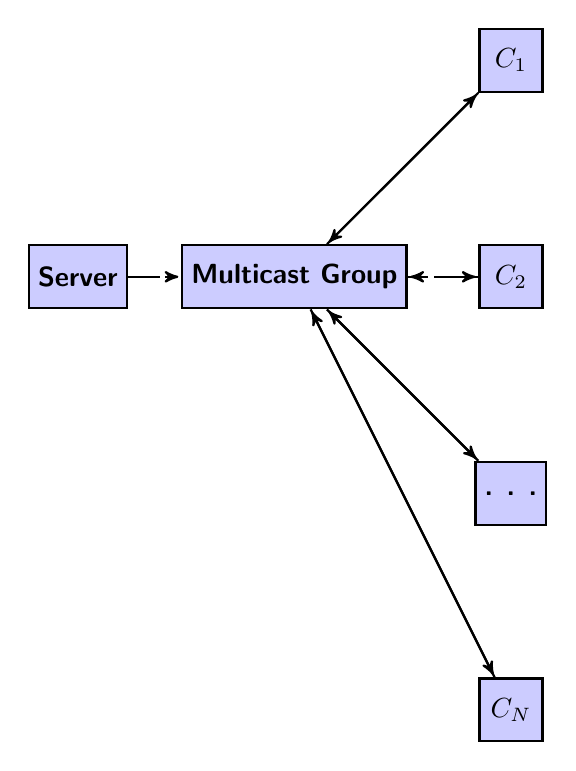
\begin{tikzpicture}[->,>=stealth',shorten >=1pt,auto,node distance=2.75cm,
  thick,main node/.style={rectangle,fill=blue!20,draw,
  font=\sffamily\bfseries,minimum size=8mm}]

  \node[main node] (MCG) {Multicast Group};
  \node[main node] (S) [left of=MCG] {Server};
  \node[main node] (Cj) [right of=MCG] {$C_{2}$};
  \node[main node] (Ci) [above of=Cj] {$C_{1}$};
  \node[main node] (dummy) [below of=Cj] {. . .};
  \node[main node] (Cn) [below of=dummy] {$C_{N}$};

  \path[every node/.style={font=\sffamily\small,
  		fill=white,inner sep=1pt}]
  		
  	%Shows Server Multicastin through group%
  	(S) edge [left=20] node[right=.5mm] {} (MCG)
    
    %Shows connection between each client and Multicasting Group%
    %Group to C1%
    (MCG) edge [] node[left=1mm] {} (Ci)
    (Ci) edge [] node[left=1mm] {} (MCG)
    %Group to C2%
    (MCG) edge [] node[left=1mm] {} (Cj)
    (Cj) edge [] node[left=1mm] {} (MCG)
    %Group to dummy%
    (MCG) edge [] node[left=1mm] {} (dummy)
    (dummy) edge [] node[left=1mm] {} (MCG)
    %Group to CN%
    (MCG) edge [] node[left=1mm] {} (Cn)
    (Cn) edge [] node[left=1mm] {} (MCG);
    
	
\end{tikzpicture}
\end{document}\textsl{•}